\documentclass[10pt]{report}
\usepackage{musa, enumitem, graphicx, listings}
\begin{document}

\title{CS 285 Homework 4: Model-Based RL}
\author{Zekai Wang (SID 3038468435)}
\date{\today}
\maketitle

\section*{2. Analysis}
\subsection*{Problem 2.1}
Proof: 
\begin{align*}
	Q^\pi - \widehat{Q}^\pi &= (I - \gamma P^\pi)^{-1} r - \widehat{Q}^\pi \\
	&= (I - \gamma P^\pi)^{-1} r - (I - \gamma P^\pi)^{-1} (I - \gamma P^\pi) \widehat{Q}^\pi \\
	&= (I - \gamma P^\pi)^{-1} [(I - \gamma \widehat{P}^\pi)\widehat{Q}^\pi - (I - \gamma P^\pi)\widehat{Q}^\pi] \\
	&= \gamma (I - \gamma P^\pi)^{-1} (P^\pi - \widehat{P}^\pi) \widehat{Q}^\pi \\
	&= \gamma (I - \gamma P^\pi)^{-1} (P - \widehat{P}) \Pi \widehat{Q}^\pi \\
	&= \gamma (I - \gamma P^\pi)^{-1} (P - \widehat{P}) \widehat{V}^\pi
\end{align*}


\subsection*{Problem 2.2}
\begin{enumerate}
	\item 
	This is True

	Proof: Let $A \in \mathbb{R}^{m \times n}, b \in \mathbb{R}^n$, let $a_i$ be the i th row of $A$, then
	\begin{align*}
		\lVert Ab \rVert_\infty &= \max_{i} |\sum_{j} A_{ij} b_j| \\
		&\leq \max_i \sum_j |A_{ij}| |b_j| \\
		&\leq \max_i \sum_j |A_{ij}| \lVert b \rVert_\infty \\
		&= \lVert b \rVert_\infty \max_i \lVert a_i \rVert_1
	\end{align*}

	Plugging in $A = P - \widehat{P}, b = \widehat{V}^\pi$, we have $\lVert (P - \widehat{P}) \widehat{V}^\pi \rVert_\infty \leq \max_{s, a} \lVert P(\cdot | s, a) - \widehat{P}(\cdot | s, a)\rVert_1 \lVert \widehat{V}^\pi \rVert_\infty$, i.e. the first inequality. 

	By the "Concentration for Discrete Distributions" lemma proposed in lecture 17 (which is Proposition A.8 in the RL Theorey textbook), fix $s, a$, then $\mathbb{P}[\lVert P(\cdot | s, a) - \widehat{P}(\cdot | s, a)\rVert_1 \geq \sqrt{|\mathcal{S}|} (\frac{1}{\sqrt{N}} + \epsilon)] \leq 2e^{-N\epsilon^2}$, so
	\begin{align*}
		\mathbb{P}[\lVert (P - \widehat{P}) \widehat{V}^\pi \rVert_\infty \geq \lVert \widehat{V}^\pi \rVert_\infty \sqrt{|\mathcal{S}|} (\frac{1}{\sqrt{N}} + \epsilon)] &\leq \mathbb{P}[\max_{s, a} \lVert P(\cdot | s, a) - \widehat{P}(\cdot | s, a)\rVert_1 \geq \sqrt{|\mathcal{S}|} (\frac{1}{\sqrt{N}} + \epsilon)] \\
		&= \mathbb{P}\{\cup_{s, a} [\lVert P(\cdot | s, a) - \widehat{P}(\cdot | s, a)\rVert_1 \geq \sqrt{|\mathcal{S}|} (\frac{1}{\sqrt{N}} + \epsilon)]\} \\
		&\leq |\mathcal{S}||\mathcal{A}| 2 e^{-N\epsilon^2}
	\end{align*}
	Let $\delta = |\mathcal{S}||\mathcal{A}| 2 e^{-N\epsilon^2}$, then $\epsilon^2 = \log(\frac{2 |\mathcal{S}||\mathcal{A}|}{\delta}) / N$. Since $\frac{2\sqrt{\log(|\mathcal{S}||\mathcal{A}| / \delta)}}{\sqrt{N}} \geq \frac{1 + \sqrt{\log(2 |\mathcal{S}||\mathcal{A}| / \delta)}}{\sqrt{N}}$ for any nontrivial case
	\begin{align*}
		\mathbb{P}[\lVert (P - \widehat{P}) \widehat{V}^\pi \rVert_\infty \geq \lVert \widehat{V}^\pi \rVert_\infty \sqrt{|\mathcal{S}|}\frac{2\sqrt{\log(|\mathcal{S}||\mathcal{A}| / \delta)}}{\sqrt{N}}] &\leq \mathbb{P}[\lVert (P - \widehat{P}) \widehat{V}^\pi \rVert_\infty \geq \lVert \widehat{V}^\pi \rVert_\infty \sqrt{|\mathcal{S}|}\frac{1 + \sqrt{\log(2 |\mathcal{S}||\mathcal{A}|\delta)}}{\sqrt{N}}] \\
		&\leq \delta
	\end{align*}
	Assume $r(s, a) \in [0, 1]$ for all $s, a$, then $\lVert \widehat{V}^\pi \rVert_\infty \leq \frac{1}{1-\gamma}$, so 
	$$\mathbb{P}[\lVert (P - \widehat{P}) \widehat{V}^\pi \rVert_\infty \geq \frac{\sqrt{4 |\mathcal{S}| \log(|\mathcal{S}||\mathcal{A}| / \delta)}}{(1-\gamma) \sqrt{N}}] \leq \delta$$
	In other words we have the conclusion. 

	\item 
	This is False

	Similar to part 3, however in this case $X_i = \mathbb{I}_{s'_i} \widehat{V}^\pi$ depends on the collected $s'_1, ..., s'_N$. So $X_i$ is not just a function of $s'_i$, this means $X_1, ..., X_N$ is no longer independent, and thus we cannot apply Hoeffding's inequality. Another issue is that the expectation $\mathbb{E}[X]$ might no longer be $\widehat{P}(\cdot | s, a) \cdot \widehat{V}^\pi$ because $\widehat{V}^\pi$ depends on $X_i$ so we cannot break them apart in the calculation. 

	\item 
	This is True

	Proof: For any $s, a$, the setting is that we sample $s'_1, ..., s'_N \sim \mathbb{P}(\cdot | s, a)$ i.i.d. from the "transition" distribution conditioned on the current state and action. Using dot product, define a function $X(s') = \mathbb{I}_{s'} \cdot V^*$, here $\mathbb{I}_{s'} \in \mathbb{R}^{|\mathcal{S}|}$ is a vector of all zeros except for the $s'$ th entry, which is $1$. Let $X_i = X(s'_i)$, then $X_1, ..., X_N \sim X$ i.i.d. and $\mathbb{E}[X] = \mathbb{E}_{s' \sim \mathbb{P}(\cdot | s, a)}[\mathbb{I}_{s'} \cdot V^*] = \mathbb{E}_{s' \sim \mathbb{P}(\cdot | s, a)}[\mathbb{I}_{s'}] \cdot V^*$ because $V^*$ is a fixed vector that is independent from $s'_1, ..., s'_N$. $\mathbb{E}_{s' \sim \mathbb{P}(\cdot | s, a)} [\mathbb{I}_{s'}] = \mathbb{P}(\cdot | s, a)$, here I overload the expression $\mathbb{P}(\cdot | s, a) \in \mathbb{R}^{|\mathcal{S}|}$ such that the ith entry in $\mathbb{P}(\cdot | s, a)$ is the probability that the next state is the ith state given the current $(s, a)$. Then, $\mathbb{E}[X] = \mathbb{P}(\cdot | s, a) \cdot V^*$. Also, assume rewards $r(s, a) \in [-1, 1]$ just to get the constant right :), then $X_i \in [-\frac{1}{1-\gamma}, \frac{1}{1-\gamma}]$. Thus, by Hoeffding's indequality, 
	$$\mathbb{P}[|\frac{1}{N} \sum_i X_i - \mathbb{E}[X]| \geq \epsilon] \leq 2 e^{-2 N \epsilon^2 (1-\gamma)^2 / 4}$$
	Since $\mathbb{E}[X] = P(\cdot | s, a) \cdot V^*$, $\frac{1}{N} \sum_i X_i = \widehat{P}(\cdot | s, a) \cdot V^*$, the above inequality gives us 
	$$\mathbb{P}[|(\widehat{P}(\cdot | s, a) - P(\cdot | s, a)) \cdot V^*| \geq \epsilon] \leq 2 e^{-2 N \epsilon^2 (1-\gamma)^2 / 4}$$
	for any $s, a$. 
	\begin{align*}
		\mathbb{P}[\lVert (P-\widehat{P})V^* \rVert_\infty \geq \epsilon] &= \mathbb{P}[\cup_{s, a} \{|(\widehat{P}(\cdot | s, a) - P(\cdot | s, a)) \cdot V^*| \geq \epsilon\}] \\
		&\leq \sum_{s, a} \mathbb{P}[|(\widehat{P}(\cdot | s, a) - P(\cdot | s, a)) \cdot V^*| \geq \epsilon] \\
		&\leq 2|\mathcal{S}||\mathcal{A}|e^{-2 N \epsilon^2 (1 - \gamma)^2 / 4}
	\end{align*}
	Let $\delta = 2|\mathcal{S}||\mathcal{A}|e^{-2N \epsilon^2 (1 - \gamma)^2 / 4}$, then $\epsilon = \sqrt{\frac{2}{N (1-\gamma)^2} \log(\frac{2|\mathcal{S}||\mathcal{A}|}{\delta})}$, so 
	$$\mathbb{P}[\lVert (P - \widehat{P}) V^* \rVert_\infty \geq \frac{1}{1-\gamma} \sqrt{\frac{2 \log(2|\mathcal{S}||\mathcal{A}|/\delta)}{N}}] \leq \delta$$
	In other words we have the conclusion.


	\item
	This is False

	Similar to part 3, however in this case $X_i = \mathbb{I}_{s'_i} \widehat{V}^*$ depends on the collected $s'_1, ..., s'_N$. So $X_i$ is not just a function of $s'_i$, this means $X_1, ..., X_N$ is no longer independent, and thus we cannot apply Hoeffding's inequality. Another issue is that the expectation $\mathbb{E}[X]$ might no longer be $\widehat{P}(\cdot | s, a) \cdot \widehat{V}^*$ because $\widehat{V}^*$ depends on $X_i$ so we cannot break them apart in the calculation. 
\end{enumerate}



\newpage
\section*{4. Code}
\subsection*{Problem 1}
I choose to change the num\textunderscore layers. The default setting is num\textunderscore layers = 1, hidden\textunderscore size = 32, and learning\textunderscore rate = 1e-3.
\begin{figure}[h]
	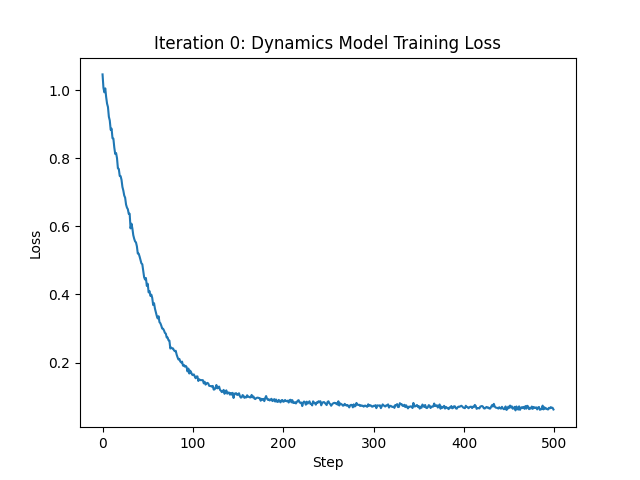
\includegraphics[width=\textwidth]{figures/Problem 1/itr_0_loss_curve_numlayers_1.png}
	\caption{num\textunderscore layers = 1}
\end{figure}
\newpage
\begin{figure}[h]
	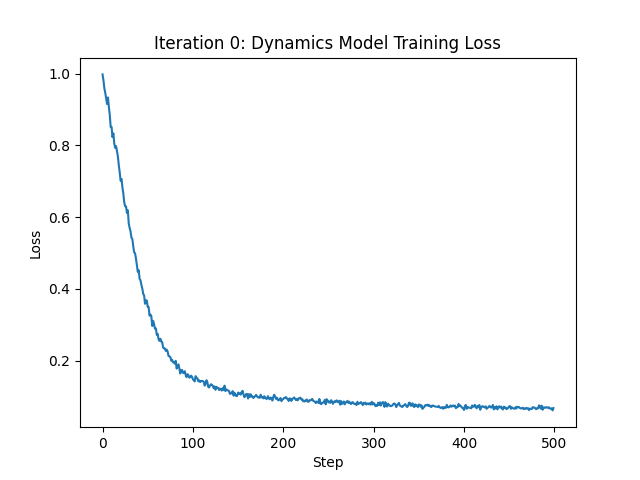
\includegraphics[width=\textwidth]{figures/Problem 1/itr_0_loss_curve_numlayers_2.png}
	\caption{num\textunderscore layers = 2}
\end{figure}
\newpage
\begin{figure}[h]
	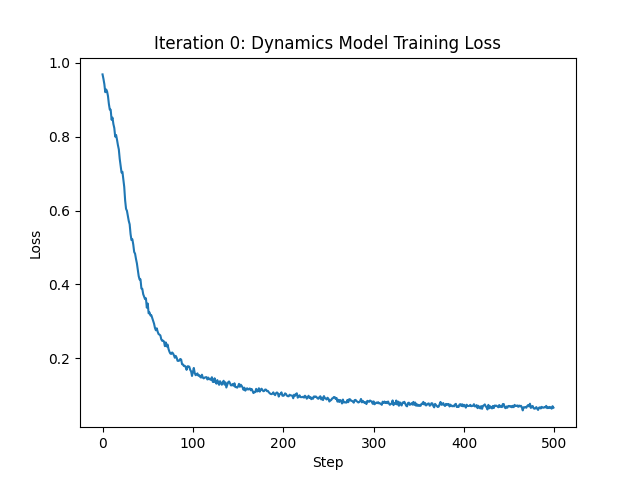
\includegraphics[width=\textwidth]{figures/Problem 1/itr_0_loss_curve_numlayers_3.png}
	\caption{num\textunderscore layers = 3}
\end{figure}

\newpage
\subsection*{Problem 2}
My eval\textunderscore return is $-37.607562544070994$.

\newpage
\subsection*{Problem 3}
\begin{figure}[h]
	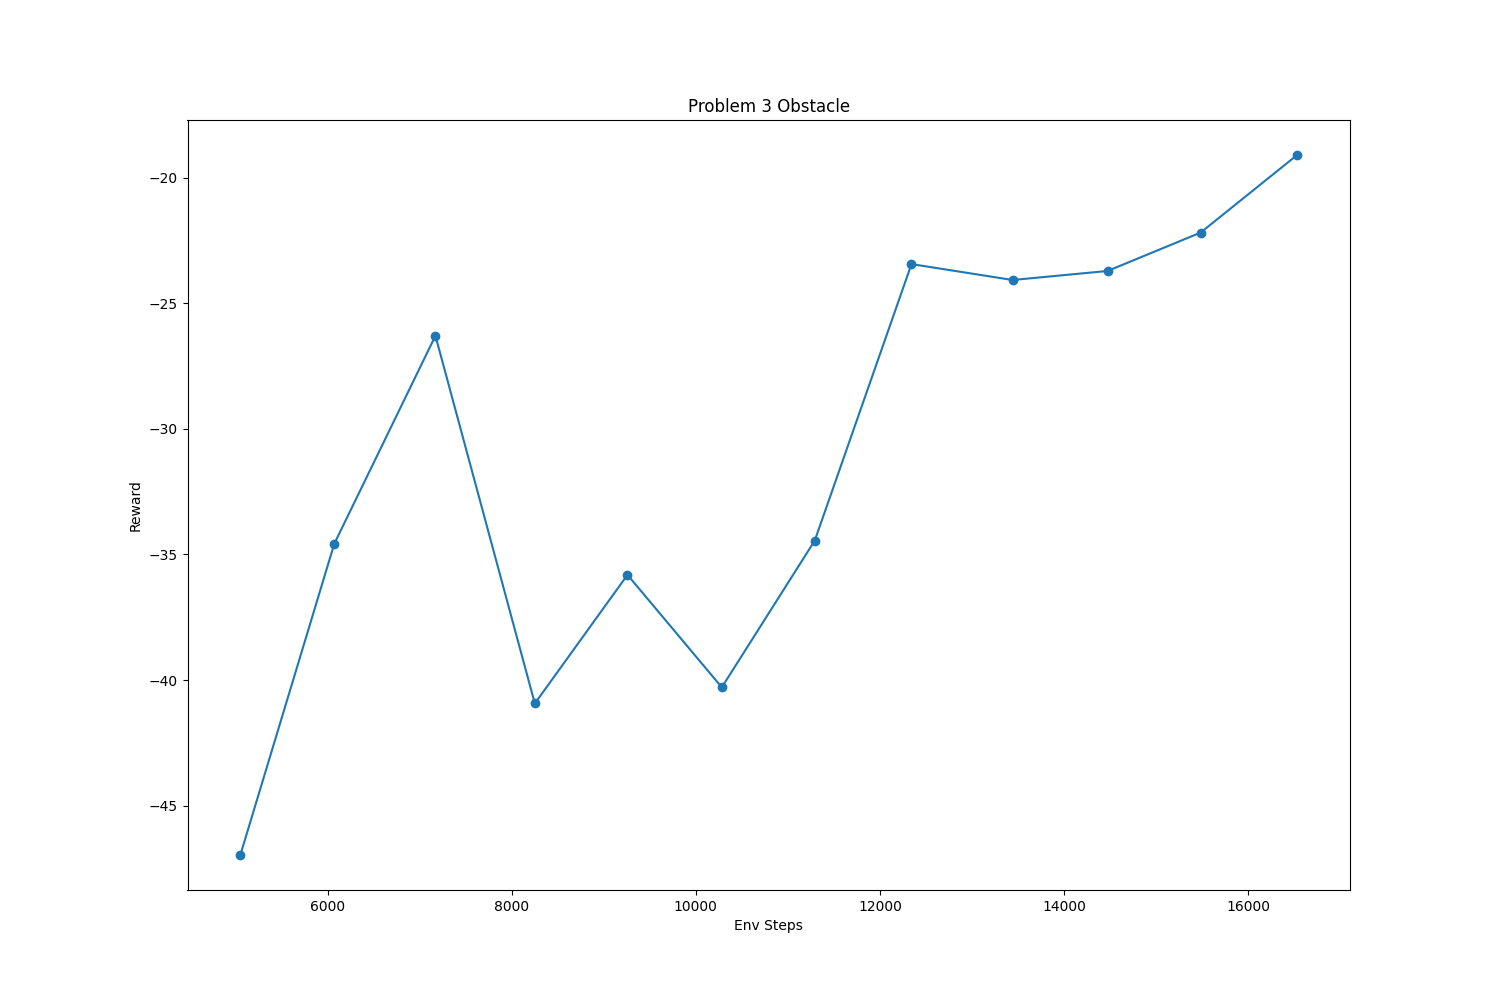
\includegraphics[width=\textwidth]{figures/Problem 3/Problem 3 Obstacle.png}
	\caption{Obstacle}
\end{figure}
\newpage
\begin{figure}[h]
	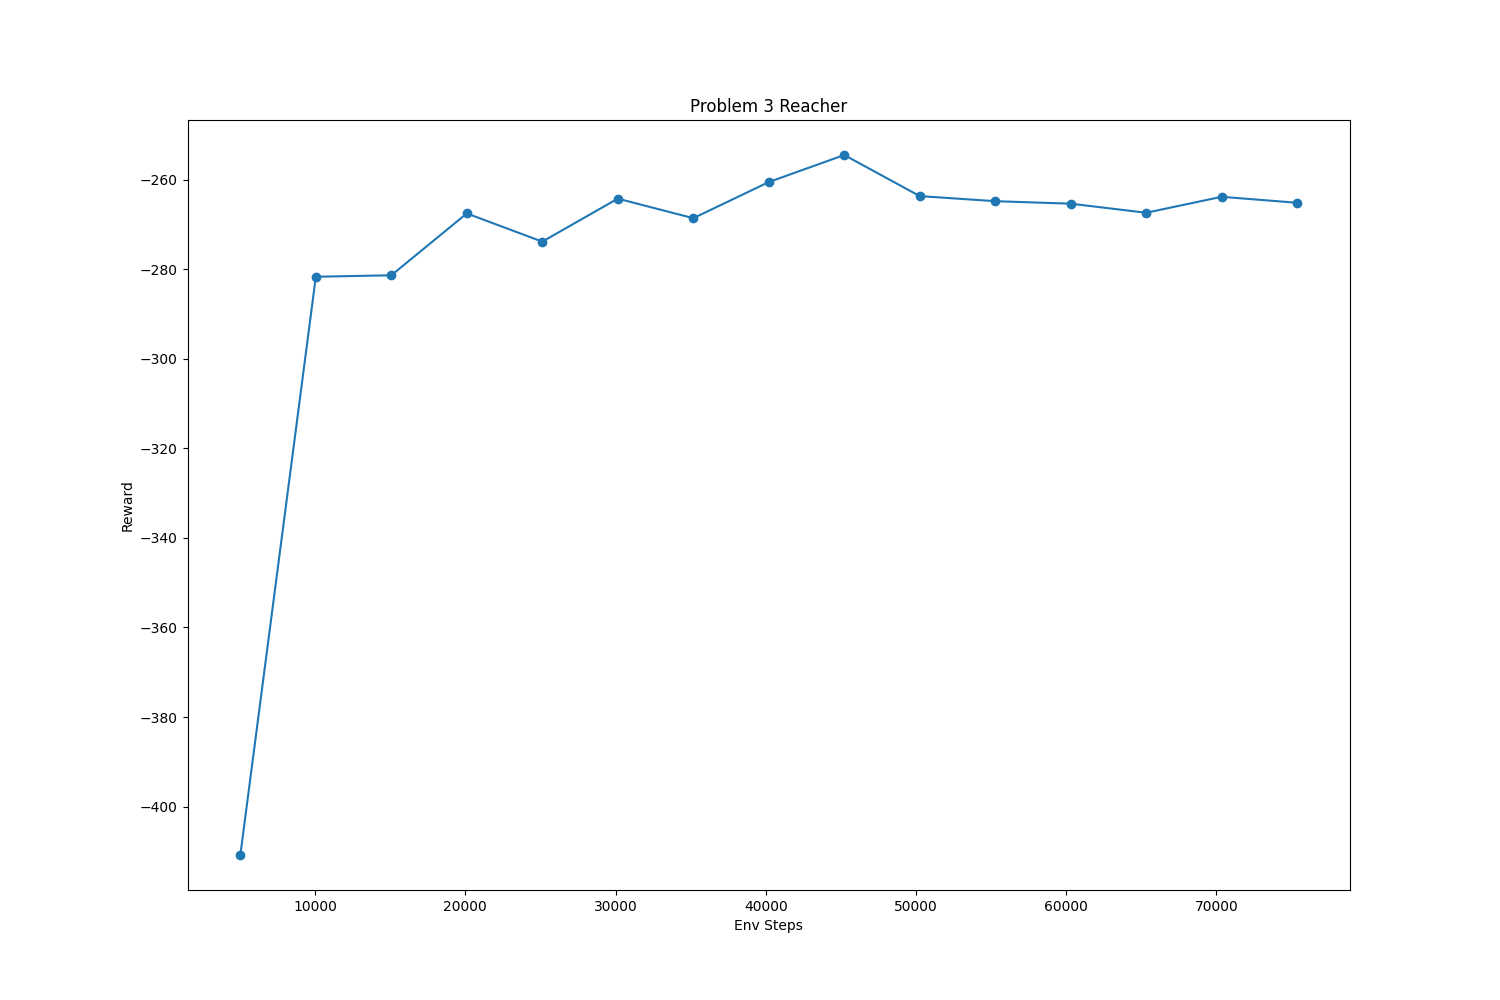
\includegraphics[width=\textwidth]{figures/Problem 3/Problem 3 Reacher.png}
	\caption{Reacher}
\end{figure}
\newpage
\begin{figure}[h]
	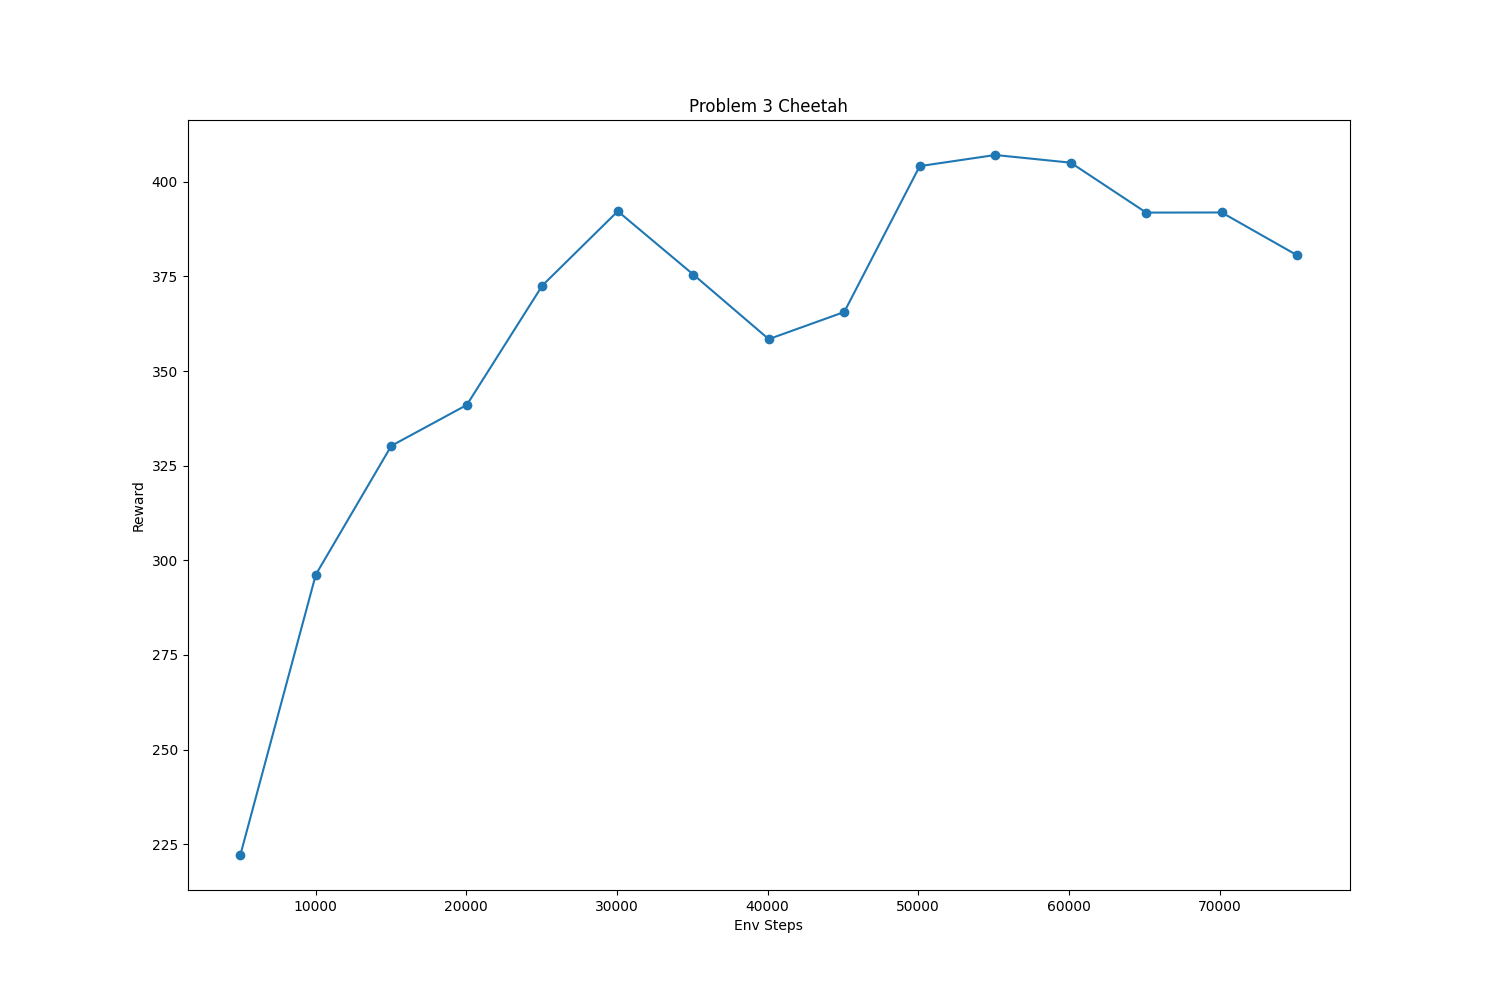
\includegraphics[width=\textwidth]{figures/Problem 3/Problem 3 Cheetah.png}
	\caption{Cheetah}
\end{figure}


\newpage
\subsection*{Problem 4}
\begin{figure}[h]
	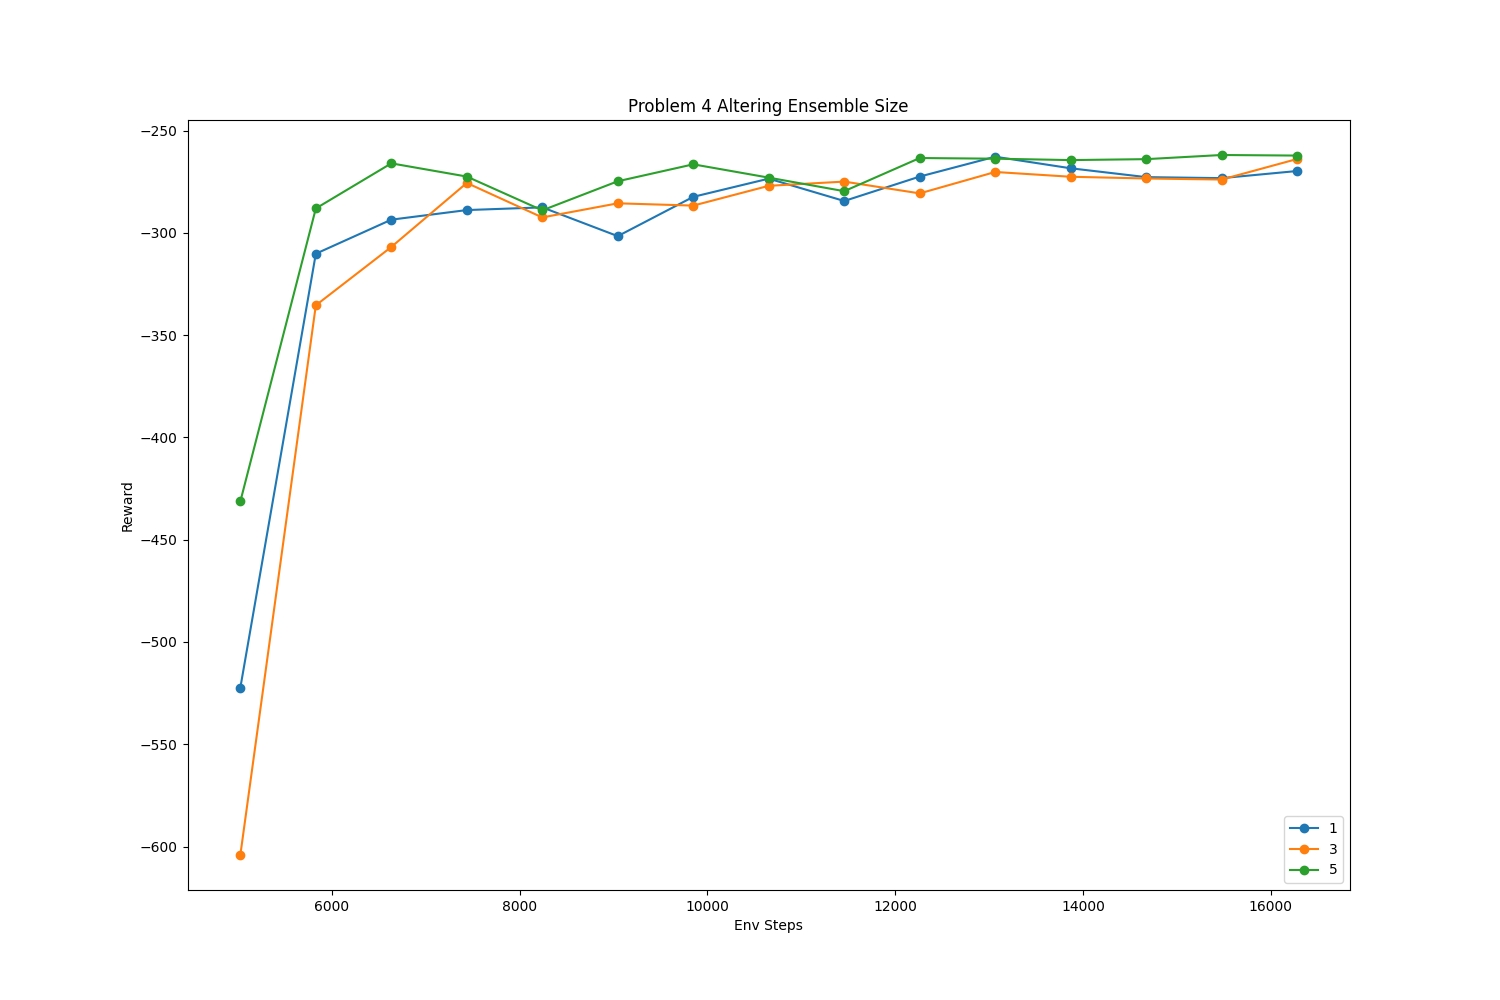
\includegraphics[width=\textwidth]{figures/Problem 4/Problem 4 ensemble.png}
	\caption{Effect of Ensemble Size, the agent tends to perform (marginally) better when the ensemble size is bigger}
\end{figure}
\newpage
\begin{figure}[h]
	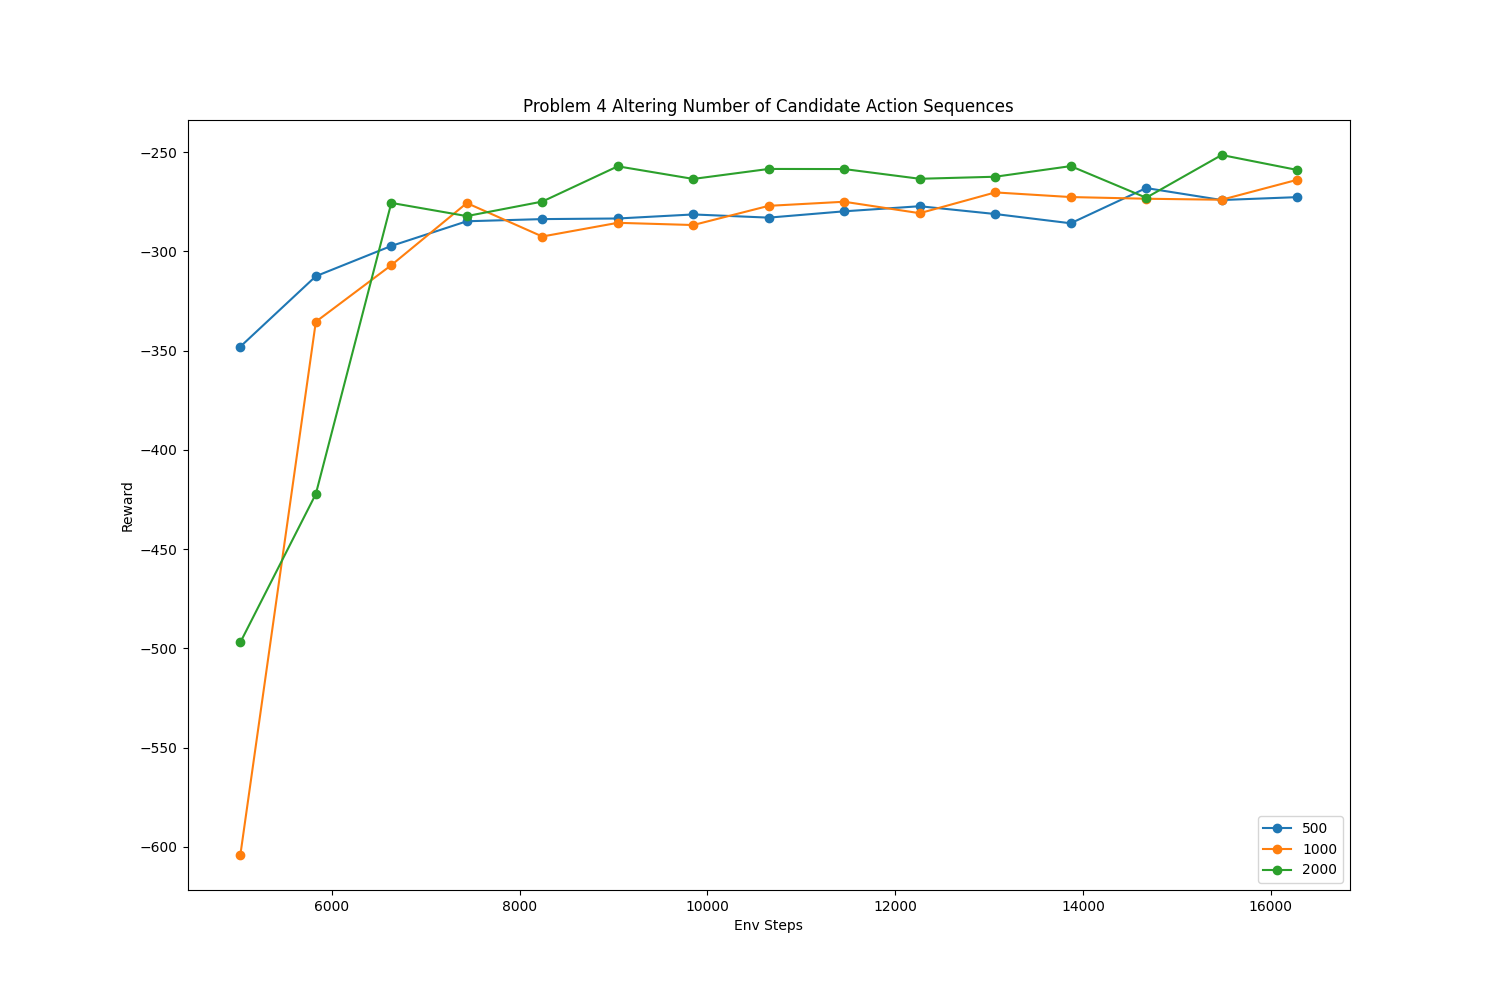
\includegraphics[width=\textwidth]{figures/Problem 4/Problem 4 numaction.png}
	\caption{Effect of the Number of Candidate Action Sequences, the agent tends to perform (marginally) better with more candidate action sequences}
\end{figure}
\newpage
\begin{figure}[h]
	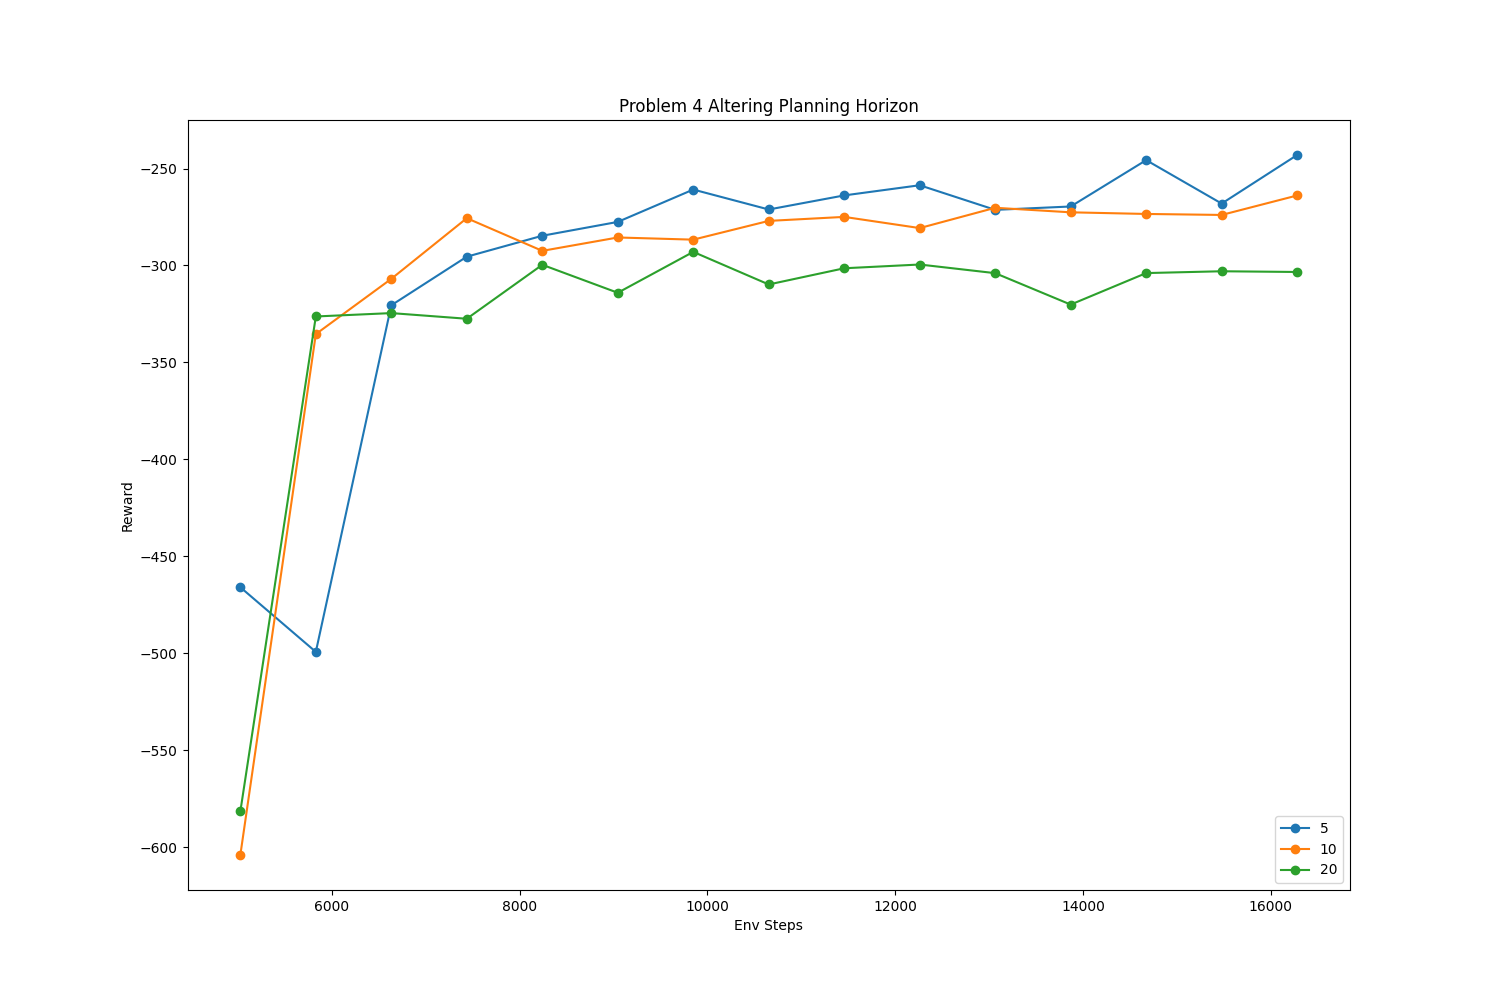
\includegraphics[width=\textwidth]{figures/Problem 4/Problem 4 horizon.png}
	\caption{Effect of Planning Horizon, the agent tends to perform better with a shorter planning horizon}
\end{figure}


\newpage
\section*{Problem 5}
\begin{figure}[h]
	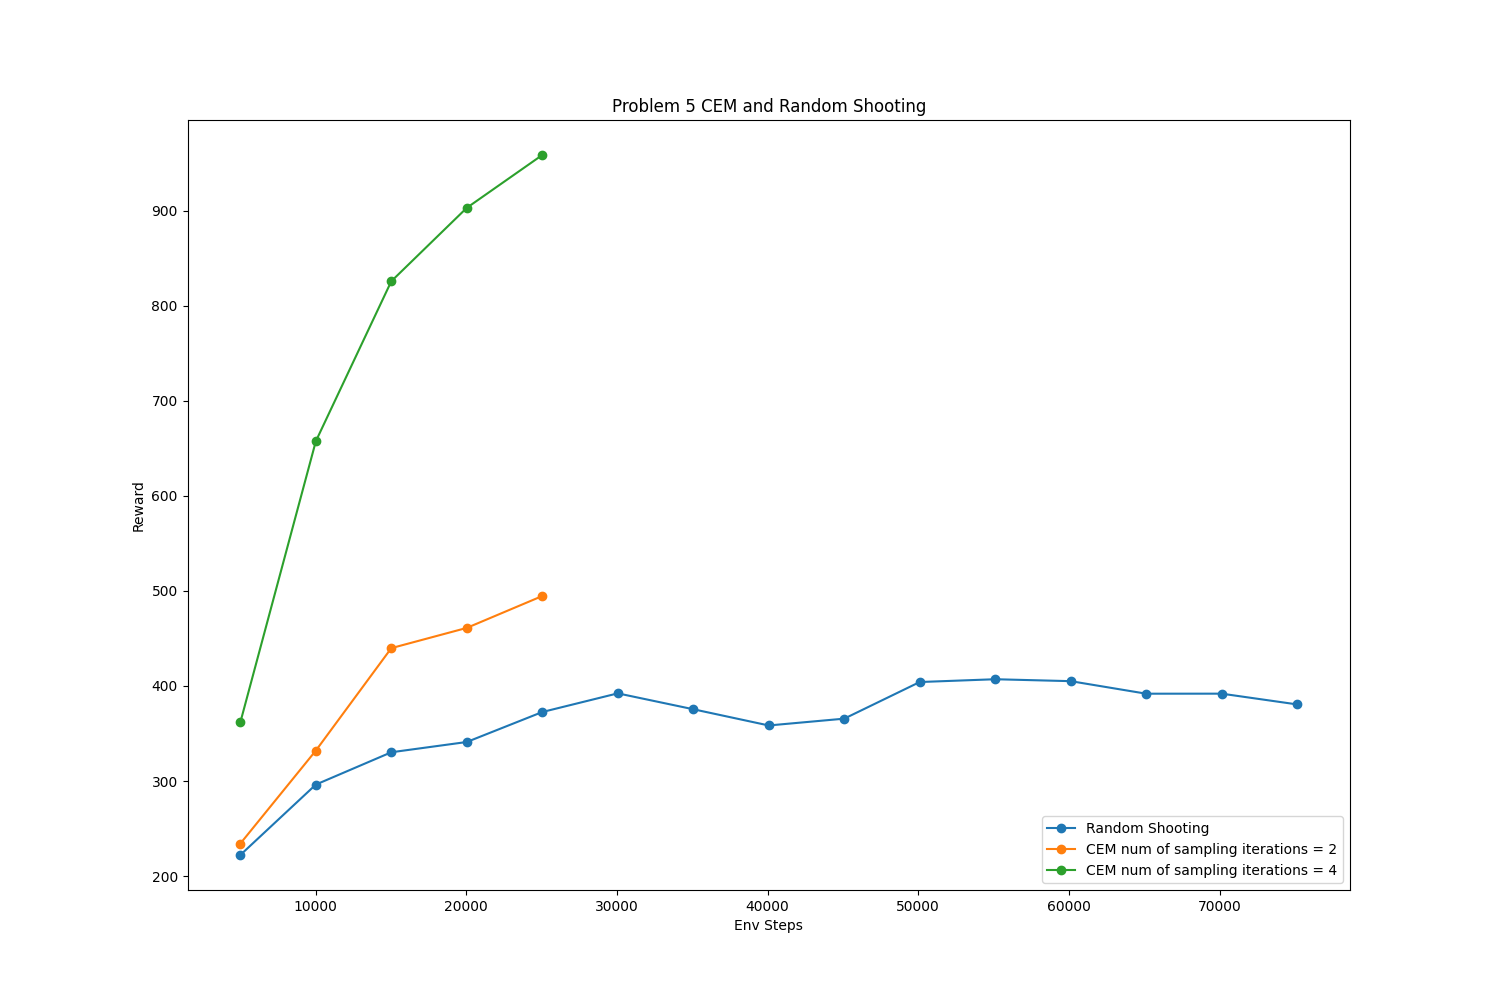
\includegraphics[width=\textwidth]{figures/Problem 5/Problem 5 cem.png}
	\caption{CEM dramatically improves the performance and efficiency of the agent. CEM with num of sampling iterations = 4 performs much better than CEM with num of sampling iterations = 2.}
\end{figure}

\newpage
\subsection*{Problem 6}
\begin{figure}[h]
	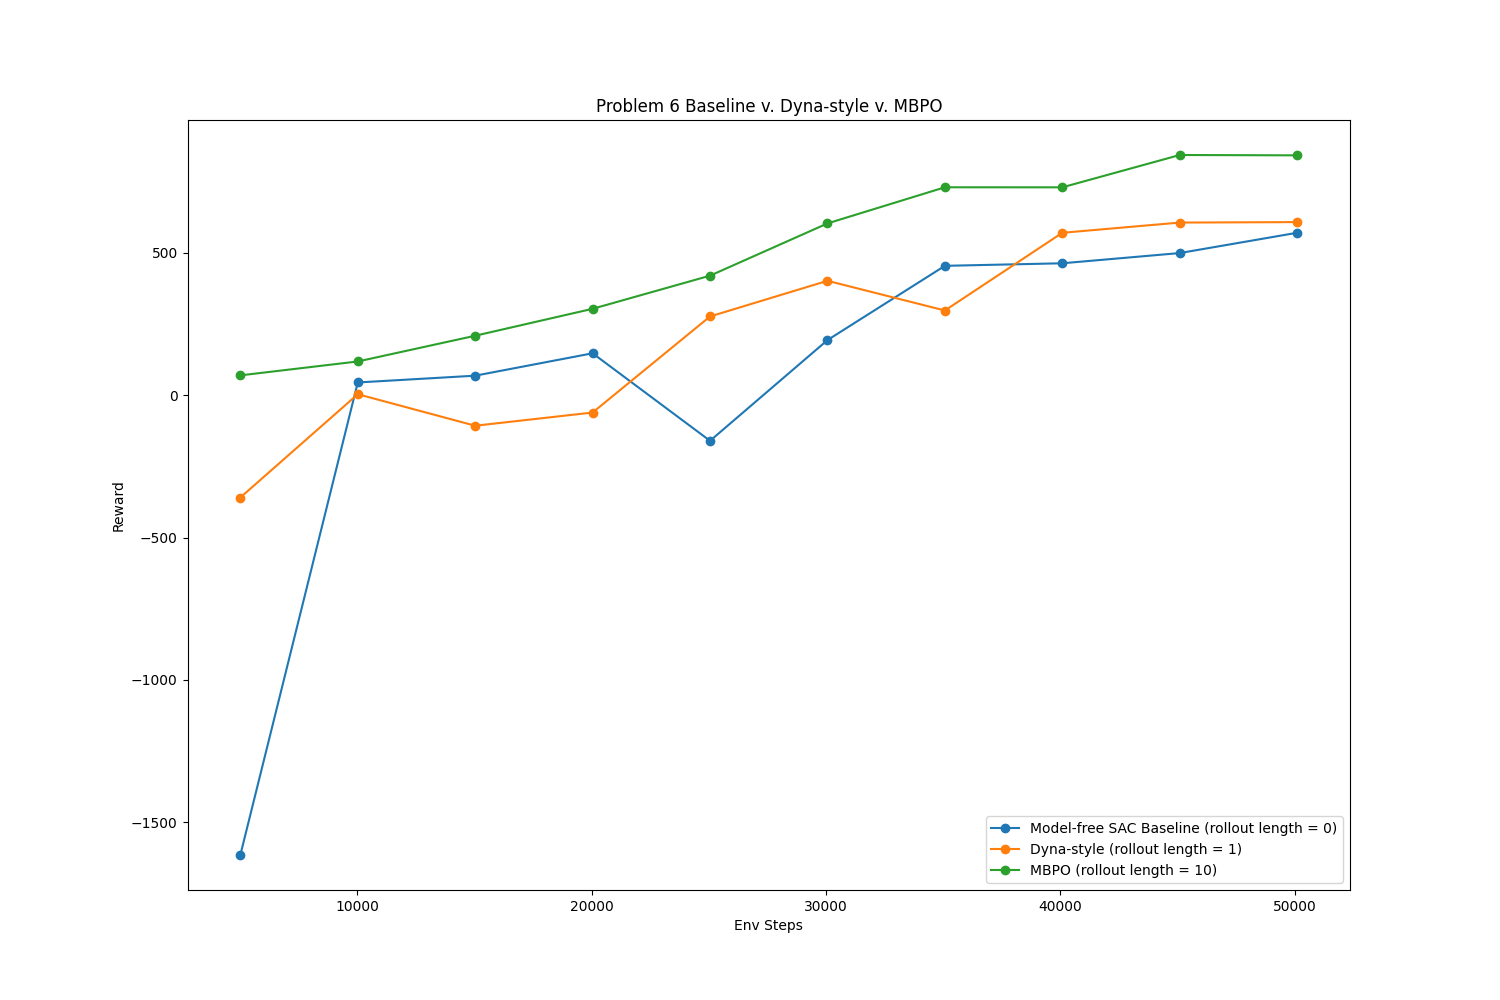
\includegraphics[width=\textwidth]{figures/Problem 6/Problem 6 mbpo.png}
	\caption{The actor tends to perform better as the rollout length increases, and SAC using mbpo performs beter than the baseline. The reason might be that when trained on a longer simulated roll-out, the SAC can consider planning on a longer horizon instead of optimizing the immediate next reward. Also, when using mbpo we can gather more simulated transitions from the leanred model to train the SAC with the same amount of environment steps, which is more efficient than gathering transitions directly from the environment. The Dyna-style agent performs marginally better than the baseline, possibly because we can train the SAC on more traisitions given the same amount of environment steps, but training it on a rollout length of 1 makes the agent prioritizing immediate reward over possibly better actions in the long run.}
\end{figure}
\end{document}